% This is samplepaper.tex, a sample chapter demonstrating the
% LLNCS macro package for Springer Computer Science proceedings;
% Version 2.21 of 2022/01/12
%
\documentclass[runningheads]{llncs}
%
\usepackage{graphicx}
\usepackage{amsmath,amssymb}
\usepackage{booktabs}
\usepackage{tabularx}
\usepackage{multirow}
\usepackage{array}
\usepackage{url}
\usepackage{hyperref}
\usepackage{cite}
\usepackage[T1]{fontenc}
\usepackage{lmodern}
\usepackage{microtype}

\usepackage{color}
\usepackage{xcolor}
\newcommand{\hl}[1]{#1}
\renewcommand\UrlFont{\color{blue}\rmfamily}
\urlstyle{rm}

% Float placement optimization
\setcounter{topnumber}{3}
\setcounter{bottomnumber}{3}
\setcounter{totalnumber}{6}
\renewcommand{\topfraction}{0.95}
\renewcommand{\bottomfraction}{0.90}
\renewcommand{\textfraction}{0.05}
\renewcommand{\floatpagefraction}{0.65}

% Float spacing optimization to prevent artificial page inflation
\setlength{\textfloatsep}{3pt plus 1pt minus 1pt}
\setlength{\floatsep}{3pt plus 1pt minus 1pt}
\setlength{\intextsep}{3pt plus 1pt minus 1pt}
\setlength{\abovecaptionskip}{2pt}
\setlength{\belowcaptionskip}{0pt}

\hypersetup{
    colorlinks=true,
    linkcolor=blue,
    filecolor=magenta,      
    urlcolor=blue,
    citecolor=blue,
}

\begin{document}
%
\title{List-Based versus Map-and-Timeline Project Information: A Pilot Study of Citizen Comprehension}
%
\titlerunning{List-Based vs. Map-and-Timeline Project Information}
%
\author{Ahmad Syifa'ul Falakhul Khayyi\inst{1} \and Aimatus Sholiha\inst{1}}
%
\authorrunning{A. S. F. Khayyi and A. Sholiha}
%
\institute{Dept. of Informatics and Computer Engineering, Politeknik Elektronika Negeri Surabaya, Surabaya, Indonesia\\
\email{khayyi@it.student.pens.ac.id, aimatus@it.student.pens.ac.id}}
%
\maketitle              % typeset the header of the contribution
%
\begin{abstract}
Public infrastructure portals predominantly display civil works in unstructured tabular lists, obscuring geographic context and inducing cognitive confusion between calendar time elapsed, physical completion, and reporting recency. This pilot study investigates whether an integrated map-and-timeline interface significantly enhances citizen comprehension compared to a list-based format. Utilizing CivicTrack, an infrastructure monitoring platform for Lamongan Regency, Indonesia, we benchmarked 20 municipal projects across a three-phase empirical evaluation. Study~1 validated baseline data integrity. Study~2 executed a counterbalanced within-subjects crossover experiment ($N = 16$) across four core retrieval tasks. Study~3 evaluated user interpretation of stale and missing progress data. The results reveal a task-dependent dichotomy. Interactive geospatial maps significantly accelerated spatial retrieval (median 14.05\,s vs. 29.75\,s; paired $t(15) = 5.57, p < 0.001$), accompanied by a descriptive accuracy gain from 81.2\% (13/16) to 100.0\% (16/16) (exact McNemar $p = 0.250$). For schedule delay detection, chronological timelines with explicit variance cues significantly reduced completion time (median 27.70\,s vs. 44.65\,s; paired $t(15) = 5.72, p < 0.001$), elevating delay identification accuracy from 50.0\% (8/16) to 93.8\% (15/16) (exact McNemar $p = 0.016$) by mitigating the duration-work equivalence heuristic. Conversely, for isolated attribute lookup, tabular lists were significantly faster (median 12.35\,s vs. 23.85\,s; paired $t(15) = -5.05, p < 0.001$), with descriptive accuracy favoring the list format (93.8\% vs. 81.2\%; exact McNemar $p = 0.625$), exposing multi-view interaction overhead. In missing data evaluations, 31.2\% misattributed missing values to project cancellation. Civic platforms must couple spatial overviews with frictionless tabular inspection.

\keywords{Civic Technology \and Public Dashboard \and Geospatial Visualization \and Usability Evaluation \and Open Data.}
\end{abstract}
%
%
%
\section{Introduction}
Civic engagement in public infrastructure governance is essential for transparent, accountable, and participatory regional development~\cite{ansari2022enhancing,chokki2022engaging}. Across emerging administrations, municipal authorities allocate major capital budgets to road resurfacing, flood canals, bridges, and primary healthcare centers~\cite{saelawong2024transparency}. Citizens have an immediate stake in tracking these public works to plan daily transit, evaluate municipal delivery, and verify fiscal accountability~\cite{nikiforova2021open,zhao2023digital}. However, citizens seeking to locate projects and track execution confront pervasive information barriers~\cite{ansari2022enhancing,nikiforova2021open}.

As documented in international open data portals~\cite{matheus2021design,zhao2023digital}, statutory disclosures in regional contexts such as Lamongan Regency, East Java---published via municipal e-procurement (LPSE Kabupaten Lamongan)~\cite{jaelani2024pelaksanaan} and official open data (Satu Data Lamongan)~\cite{satudatalamongan2024} (\url{https://satudata.lamongankab.go.id}, accessed 15 October 2024)---sequester public works data in static tabular registries and PDF tenders. These legacy formats strip away spatial proximity, requiring citizens to manually parse hundreds of rows without an intuitive means to identify projects in their neighborhood or verify physical progress on the ground.

Beyond generic usability hurdles~\cite{nikiforova2021open,zhao2023digital}, preliminary field inquiry in Lamongan (Study~0, Section~3.5; 12 civic community members, Aug--Sept 2024) revealed two acute cognitive breakdowns:
\begin{enumerate}\setlength{\itemsep}{0.8pt}\setlength{\parskip}{0pt}
    \item \textbf{Duration-as-Progress Fallacy:} 9 of 12 participants conflated elapsed calendar time with physical progress. When inspecting a project showing `75\% elapsed time'' alongside `60\% physical progress,'' citizens inferred it was on track, overlooking a 15\% execution delay due to heuristic substitution under mismatched tabular displays~\cite{bacic2022advancing}.
    \item \textbf{Stale and Missing Data Ambiguity:} Disclosures lacked visual freshness cues. Progress updates lagging by 3--5 months left citizens unable to discern whether works were ongoing or abandoned; missing fields were often misattributed to project cancellation, mirroring negative default inferences~\cite{fernstad2022explore}.
\end{enumerate}

While municipal portals increasingly adopt visual dashboards~\cite{ansari2022enhancing,chokki2022engaging}, implementations are frequently driven by aesthetic gloss rather than cognitive task fit~\cite{chokki2022engaging,nikiforova2021open}. Uncalibrated interactive map layers introduce navigation friction (panning, zooming, marker occlusion) that degrades simple attribute lookup performance~\cite{bina2023incorporating,duncan2021task}.

To address this gap, this study proposes and evaluates \textbf{CivicTrack}, an open infrastructure monitoring platform grounded in Cognitive Fit Theory~\cite{bina2023incorporating,bacic2022advancing}. CivicTrack harmonizes an interactive geospatial map (spatial scoping), a dual-progress timeline (decoupling contractual duration from milestone completion with freshness indicators), and a filterable tabular view (direct lookup). Utilizing a 20-project benchmark modeled on Lamongan Regency, this paper presents three contributions:
\begin{enumerate}\setlength{\itemsep}{0.8pt}\setlength{\parskip}{0pt}
    \item A mathematical formulation decoupling milestone completion ($P_{physical} = \sum_{k=1}^m w_k \cdot c_k$) from duration ($T_{elapsed}$) with an unambiguous variance metric ($\Delta$) and priority rules.
    \item A counterbalanced within-subjects crossover pilot experiment ($N = 16$) separating completion time (paired $t$-tests) from binary accuracy (exact McNemar tests) across four tasks.
    \item An empirical assessment of citizen cognitive interpretations under missing and stale reporting conditions, yielding design principles for civic transparency.
\end{enumerate}

\section{Related Work}
Public project dashboard comprehension intersects four domains: open government usability, cognitive fit, geospatial civic analytics, and temporal progress tracking.

\subsection{Public Project Dashboards and Citizen Comprehension}
Digital portals aim to mitigate information asymmetry between public bodies and citizens~\cite{ansari2022enhancing,chokki2022engaging,kempeneer2023rethinking}. However, empirical audits show that raw disclosures fail to provide civic utility unless supported by task-tailored interfaces~\cite{ansari2022enhancing,matheus2021design}. Nikiforova and McBride~\cite{nikiforova2021open} observed that most portals remain passive `data dumps'' of static tables that deter non-expert inquiry. While dashboards can improve comprehension, crowded layouts risk visual fragmentation and cognitive fatigue~\cite{chokki2022engaging,zhao2023digital,kempeneer2023rethinking}.

\subsection{Cognitive Fit Theory and Visualization Usability}
Cognitive Fit Theory, recently extended for visual analytics by Bina et al.~\cite{bina2023incorporating} and Ba{\v{c}}i{\'c} and Henry~\cite{bacic2022advancing}, posits that problem-solving performance is maximized when representation matches task type: spatial inquiries benefit from graphical displays, whereas discrete lookups are best served by structured alphanumeric tables~\cite{bina2023incorporating,bacic2022advancing}. However, multi-view interfaces impose cognitive switching costs during coordinated exploration~\cite{bacic2022advancing}.

\subsection{Geospatial Visualization versus Tabular List Presentations}
Cartographic analytics distinguishes elementary tasks (locating discrete attributes of known entities) from synoptic tasks (discerning spatial clusters)~\cite{duncan2021task}. Maps excel at synoptic synthesis, whereas structured tables minimize retrieval costs for discrete attribute lookup by eliminating map navigation friction (panning, zooming, marker occlusion)~\cite{duncan2021task}. In public participation GIS (PPGIS), lay citizens frequently encounter usability friction when interpreting dense multi-layer displays~\cite{kytta2023prioritizing,johnson2024enhancing}.

\subsection{Timeline Usability and Schedule Representation}
Visualizing civil works progress requires conveying durations, milestones, and temporal pacing. Reconstructing schedule overlaps from spreadsheet dates imposes high working memory loads~\cite{tang2024comparative,bacic2022advancing}. In construction management, Ayalew and Ayalew~\cite{ayalew2024developing} demonstrated that measuring physical progress against planned schedule baselines requires explicit variance tracking rather than simplistic duration comparisons.

\subsection{Interpretation of Missing and Stale Governance Data}
Public infrastructure monitoring suffers frequently from reporting latency. Displays that omit explicit indicators for missing data lead citizens to assume administrative failure or cancellation~\cite{fernstad2022explore}. In infrastructure governance, Ambituuni~\cite{ambituuni2025infrastructure} and Saelawong et al.~\cite{saelawong2024transparency} examined the Infrastructure Transparency Initiative (CoST) through principal-agent theory, showing that open disclosures fail to generate accountability without timely, reliable data.

\subsection{Research Gap and Positioning}
Prior studies evaluate dashboard usability~\cite{ansari2022enhancing,matheus2021design,nikiforova2021open}, participatory mapping~\cite{kytta2023prioritizing,johnson2024enhancing}, or timeline modeling~\cite{ayalew2024developing} in isolation. No study empirically compares all three representations within a counterbalanced task battery on real municipal works while assessing how citizens interpret stale data. We bridge this gap by grounding CivicTrack in Cognitive Fit Theory~\cite{bina2023incorporating,bacic2022advancing}.

\section{Methodology}

\subsection{Research Question and Differentiated Hypotheses}
This study investigates the following primary research question: \emph{Does an integrated map-and-timeline interface (CivicTrack, including its explicit variance cues) improve citizen accuracy and efficiency in understanding project locations, physical progress, and schedule delays compared to a conventional list-based presentation?}

Because completion time (continuous ratio variable, seconds) and comprehension accuracy (paired binary outcome, 0/1) represent distinct operational dimensions evaluated under separate statistical tests (paired $t$-tests and exact McNemar tests, respectively), we formulate separated operational hypotheses:
\begin{itemize}\setlength{\itemsep}{1.2pt}\setlength{\parskip}{0pt}
    \item \textbf{$H_1$ (Spatial Scoping):} For spatial discovery tasks, the map interface will achieve significantly shorter completion times ($H_{1a}$) and higher descriptive or statistical retrieval accuracy ($H_{1b}$) by eliminating serial scanning fatigue.
    \item \textbf{$H_2$ (Schedule Pacing):} \hl{For schedule delay detection, the CivicTrack timeline condition (a dual-bar timeline bundled with explicit variance cues and delay badges) will yield significantly faster completion times ($H_{2a}$) and significantly higher delay identification accuracy ($H_{2b}$) than the list condition, which exposes the same underlying numeric fields but no derived variance indicator; the design does not isolate the timeline graphic from the delay badge.}
    \item \textbf{$H_3$ (Discrete Lookups):} For discrete metadata lookups (latest field update date), the tabular list will achieve significantly faster response times ($H_{3a}$) and superior descriptive accuracy ($H_{3b}$) due to the absence of multi-view spatial navigation overhead.
\end{itemize}

\subsection{System Architecture and Technical Stack}
The empirical evaluation was conducted using \textbf{CivicTrack}, an end-to-end municipal infrastructure monitoring platform engineered for the 27 subdistricts (\emph{kecamatan}) of Lamongan Regency, East Java. The technical stack comprises: (1)~\textbf{Backend Services} engineered in Python 3.11 with FastAPI for REST endpoints, Pydantic v2 schema validation, and SQLite/PostgreSQL for relational spatial storage; (2)~\textbf{Frontend Application} built in React 18, TypeScript, and responsive CSS, integrating Leaflet.js for vector boundary rendering and marker clustering; and (3)~\textbf{Analytical Engine} calculating elapsed duration, milestone-weighted physical completion, and schedule variance ($\Delta$). Figure~\ref{fig:architecture} illustrates the system architecture, component dataflows, and verification boundaries.

\begin{figure}[!htbp]
\centering
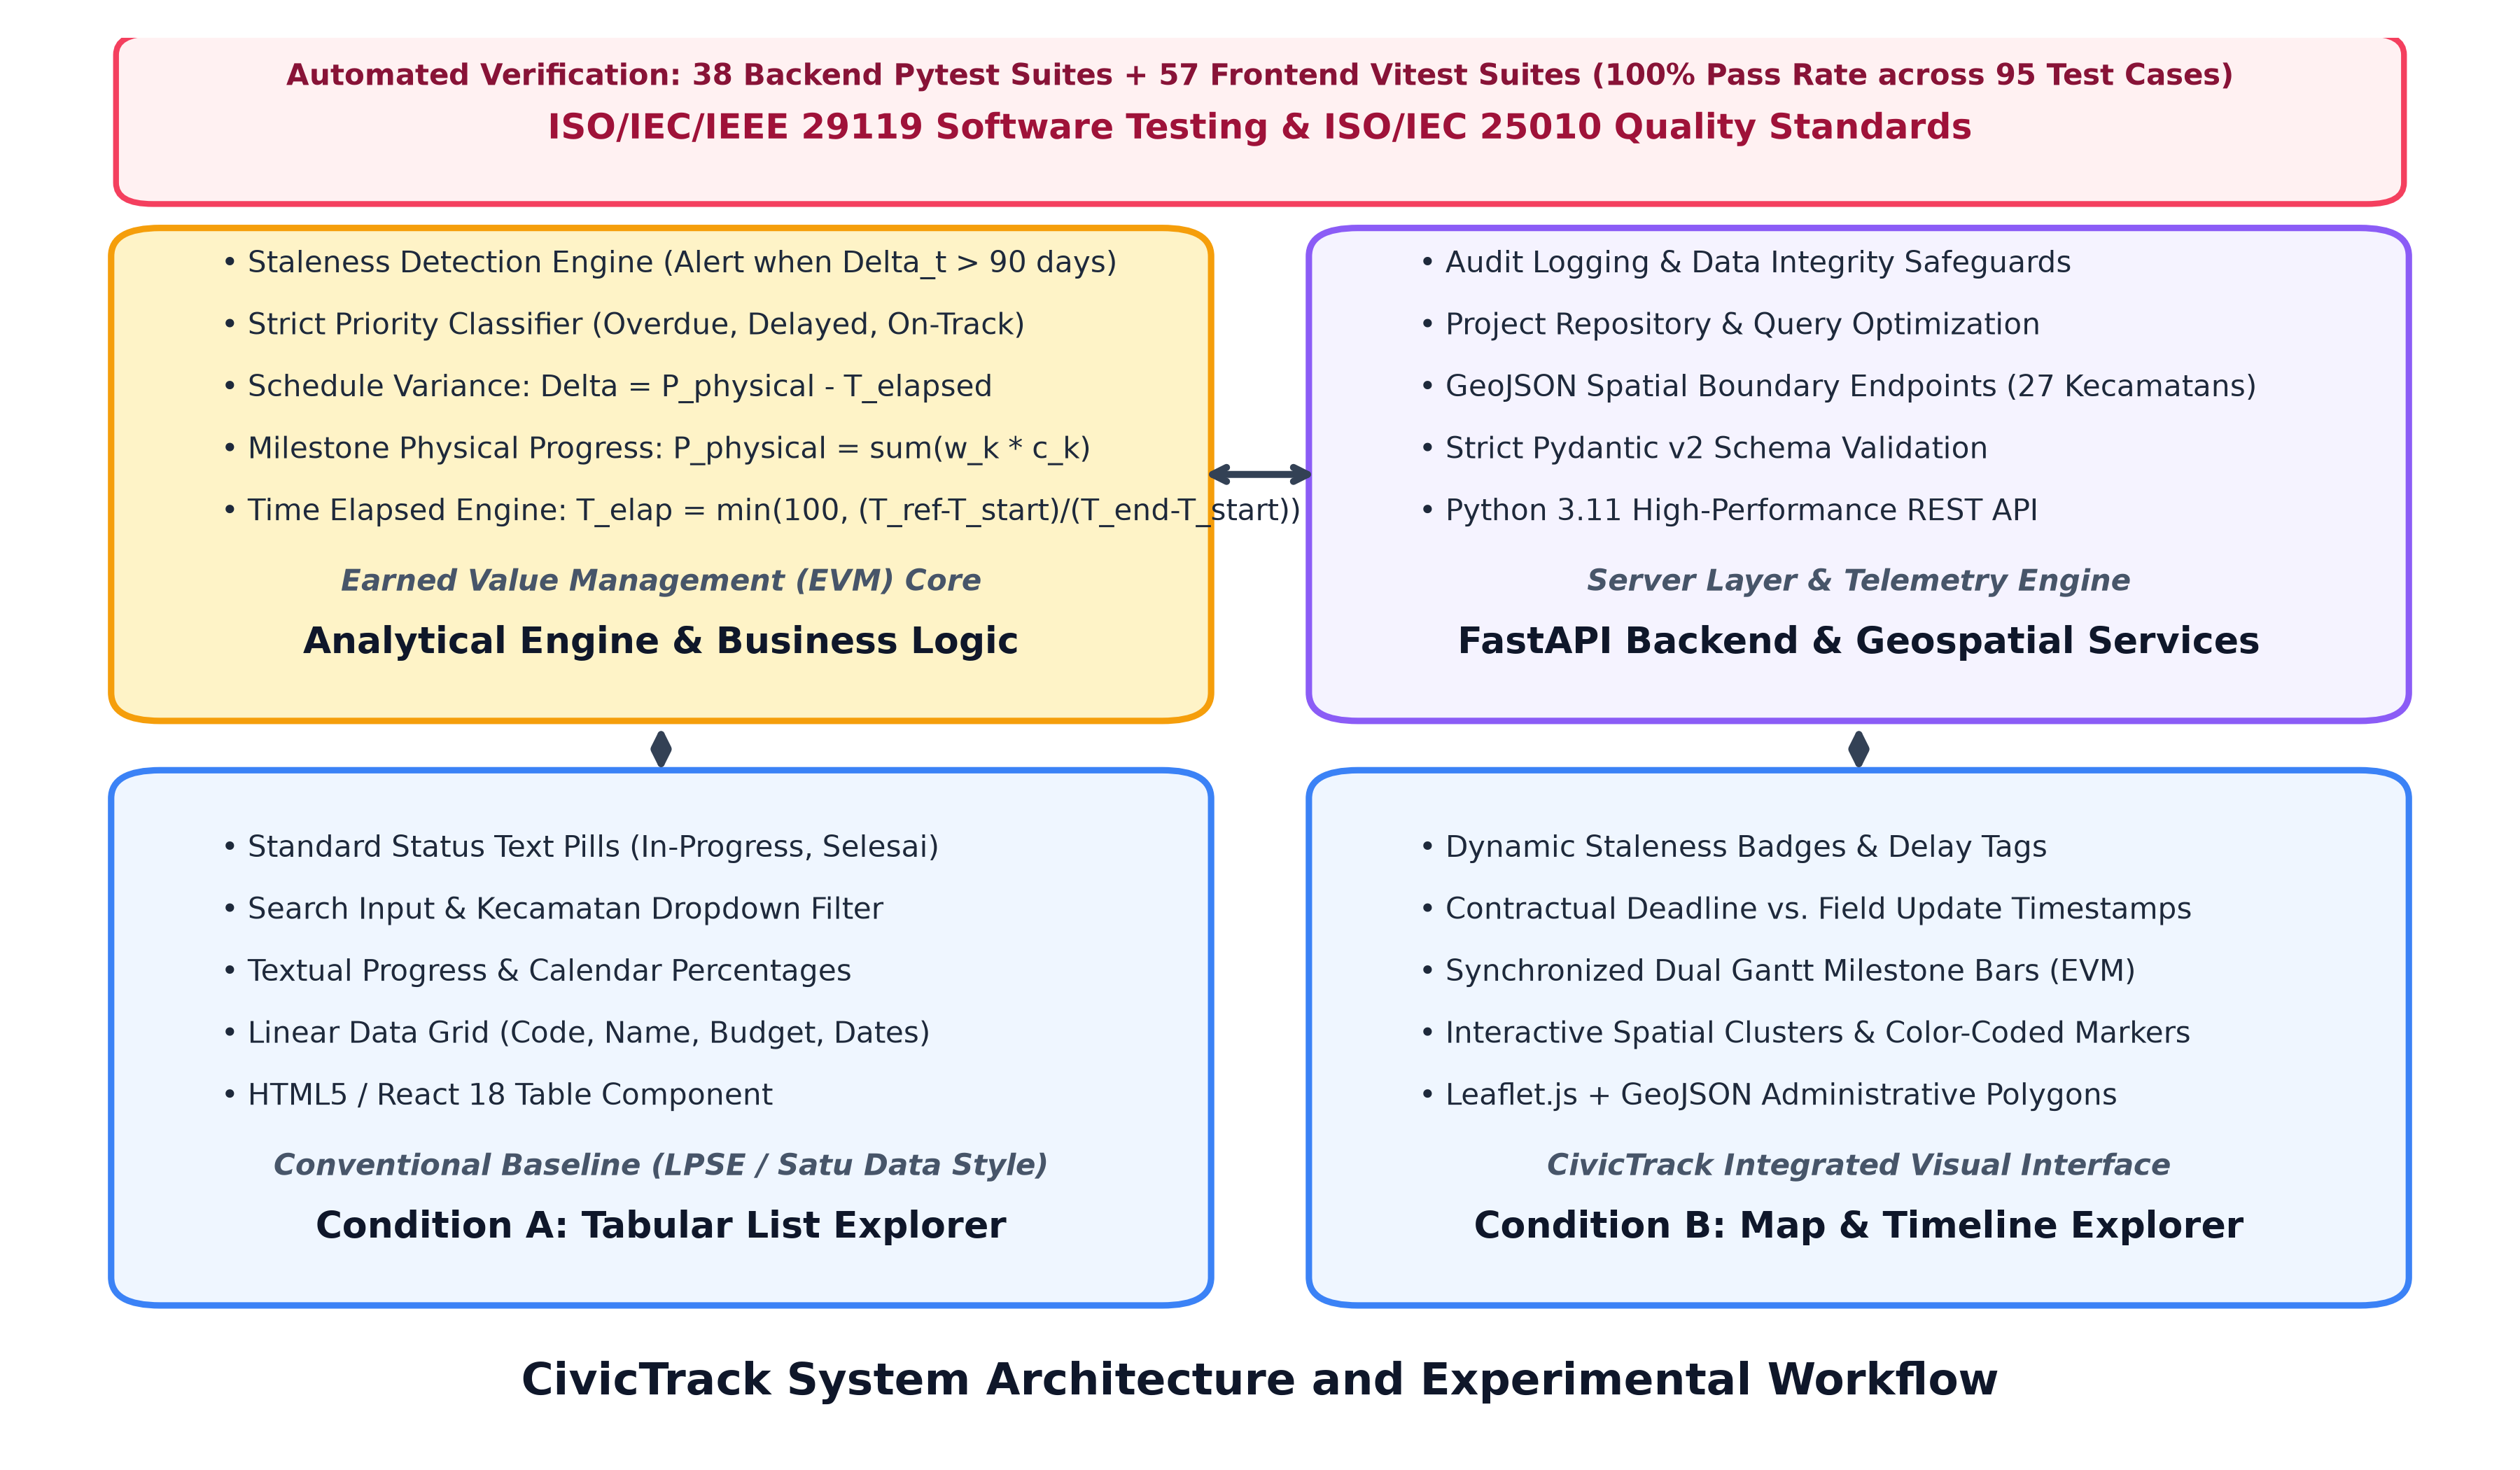
\includegraphics[width=0.60\textwidth]{figures/fig3_system_architecture.png}
\caption{CivicTrack system architecture, component dataflow, and experimental testing integration across Condition A (List View) and Condition B (Map and Timeline Explorer).}
\label{fig:architecture}
\end{figure}



\subsection{Stimulus Design and Information Parity Analysis}
To enable rigorous comparative testing, two controlled visual modalities were implemented with identical underlying project data, illustrated in Fig.~\ref{fig:comparison}:

\begin{figure}[!htbp]
\centering
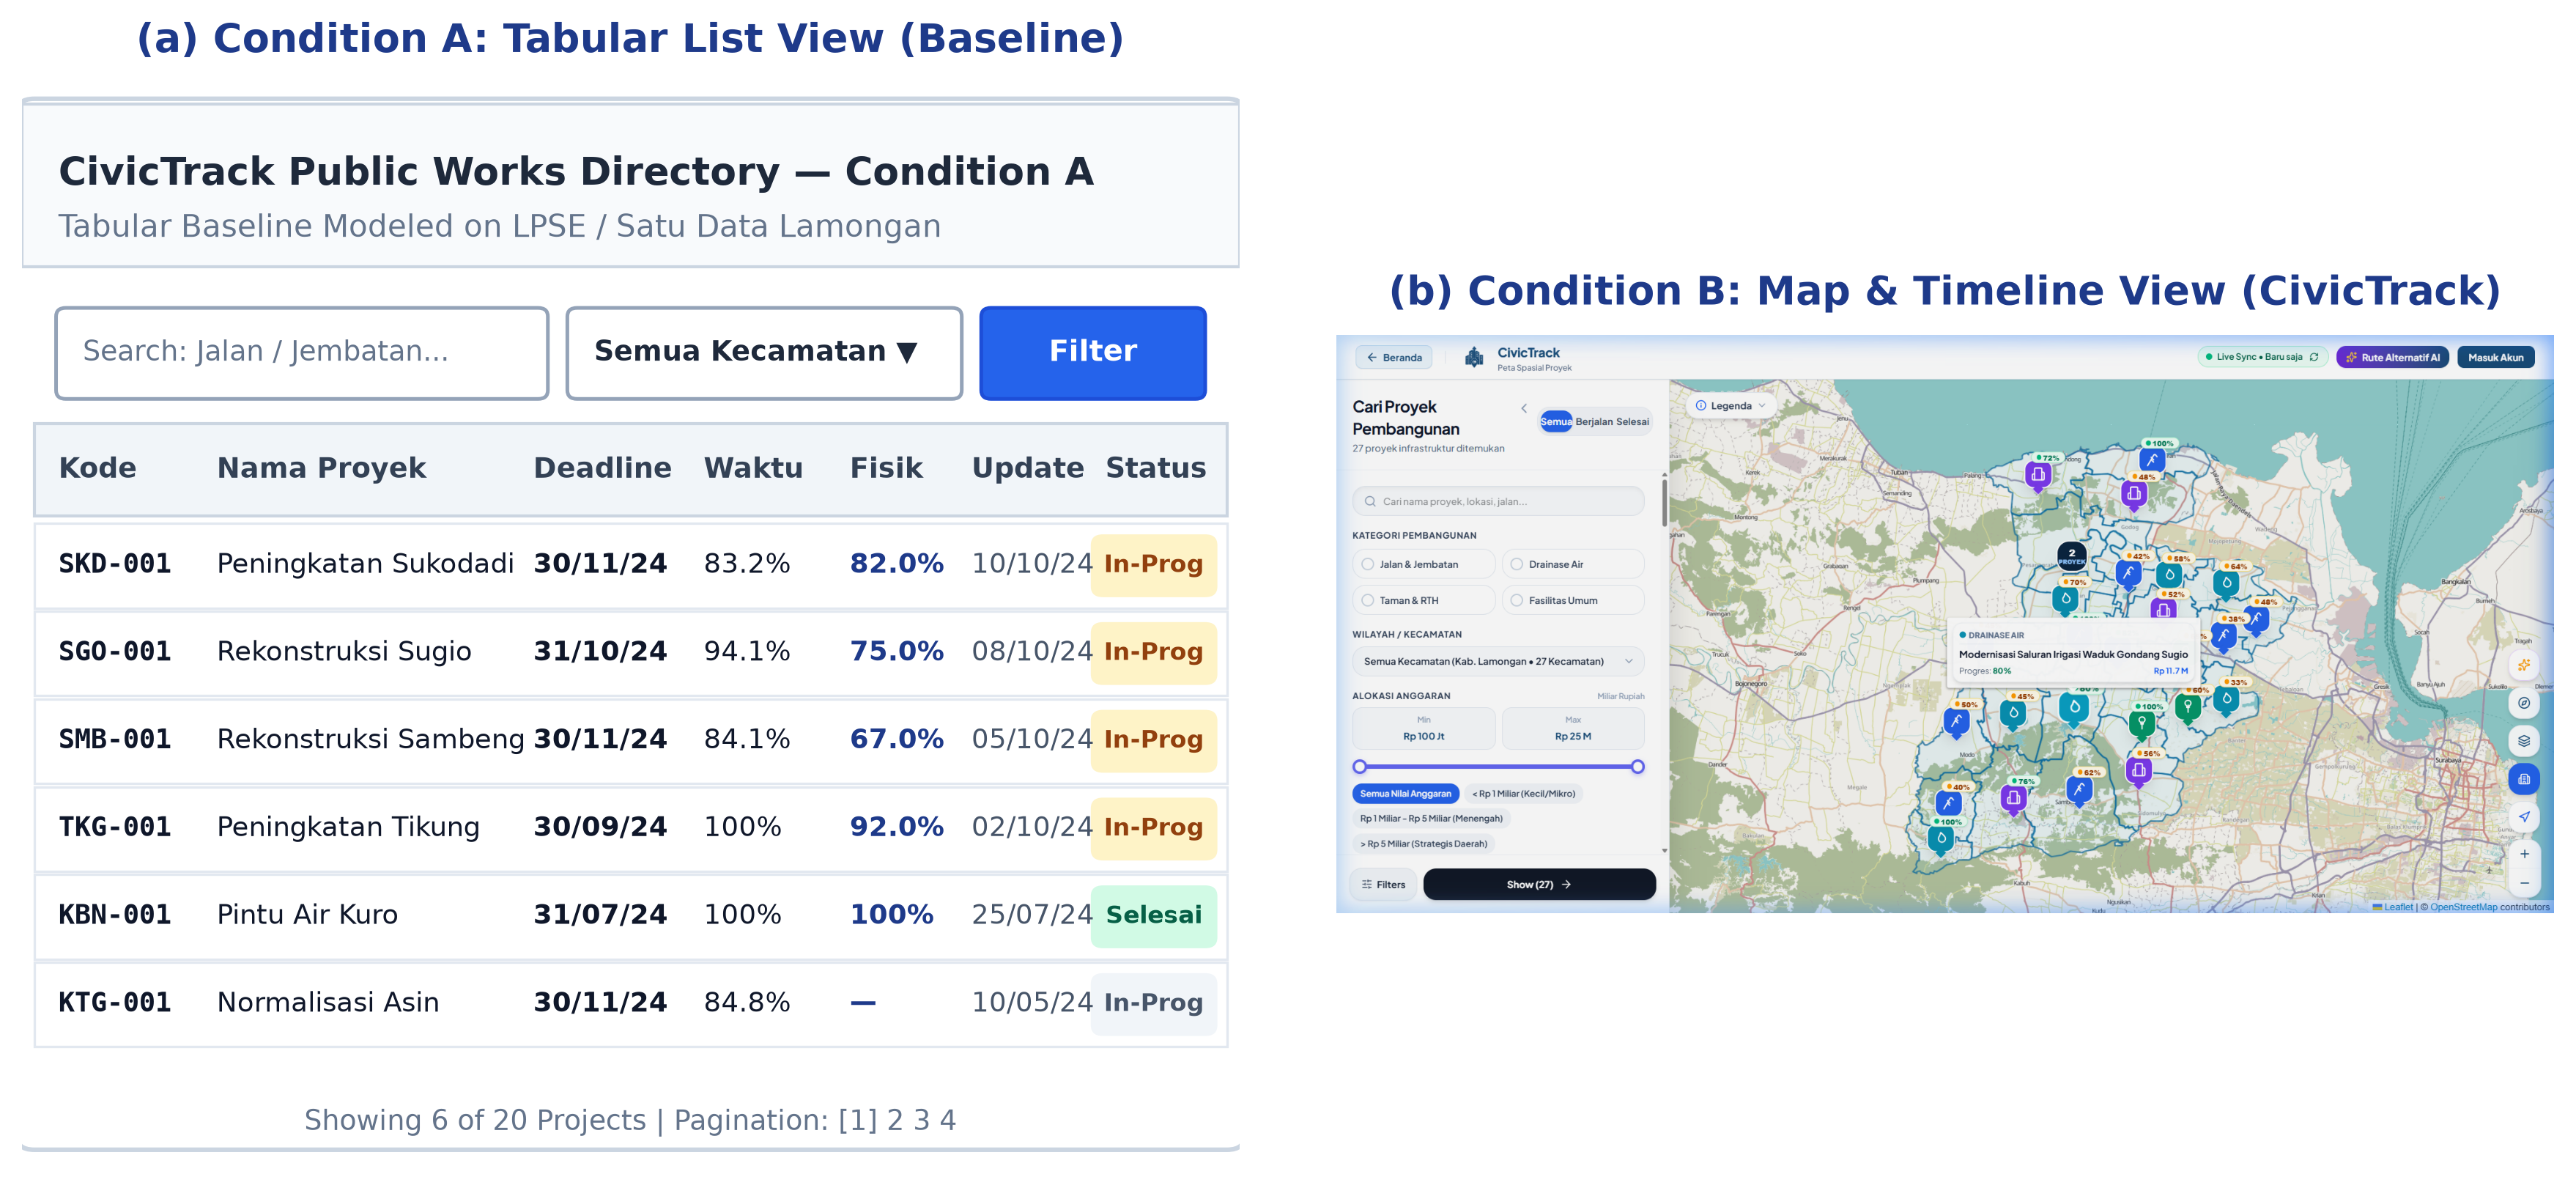
\includegraphics[width=0.62\textwidth]{figures/fig_system_interface_comparison.png}
\caption{Visual stimuli for comparative evaluation: (a) Condition A (Tabular List baseline modeled on municipal open data portals) and (b) Condition B (CivicTrack interactive Map-and-Timeline Explorer).}
\label{fig:comparison}
\end{figure}
\begin{enumerate}\setlength{\itemsep}{1.2pt}\setlength{\parskip}{0pt}
    \item \textbf{Condition A (List-Based View Baseline):} \hl{A structured, searchable, and sortable tabular presentation displaying project code, name, subdistrict, budget, contractual deadlines (for Task 3), elapsed calendar percentage, physical milestone completion percentage, latest update date, and standard status pills (``In-Progress'', ``Selesai'').}
    \item \textbf{Condition B (Map-and-Timeline Explorer):} An integrated dual-pane interactive environment. The top/left pane renders a Leaflet-based map with subdistrict boundaries and color-coded status pins (Green = Completed, Amber = On-Track, Red = Delayed, Blue = Not Started, Gray = Incomplete Data). Clicking a pin anchors the viewport and highlights the corresponding project in the bottom/right chronological timeline pane, which renders dual horizontal bars displaying scheduled baseline duration versus actual milestone completion, marked with a vertical reference line ($T_{ref} = \text{15 October 2024}$) and explicit deviation badges (e.g., ``-19.1\% Terlambat'').
\end{enumerate}



\textbf{Information Parity and Known Asymmetry:} Both interfaces provide equivalent basic tools: an alphanumeric keyword search input and a subdistrict filter dropdown. Both conditions also expose the raw numeric fields from which schedule variance can be computed (elapsed calendar percentage and physical completion percentage). However, as shown in Fig.~\ref{fig:comparison}, Condition~B visually surfaces explicit delay tags (``Terlambat'') derived from automated variance logic, whereas Condition~A displays conventional municipal portal conventions where all active projects show uniform ``In-Progress'' badges. \hl{Condition B is therefore a bundled treatment (map, dual-bar timeline, and variance cues), and differences in Tasks 2 and 4 reflect this bundle rather than the timeline graphic in isolation. This distinction mirrors real-world e-government conditions and evaluates whether citizens can detect delays from numerical columns alone versus with explicit variance cues.}

\subsection{Reference Dataset Construction (20 Synthetic Projects)}
A master benchmark dataset of 20 public infrastructure projects was synthesized directly from verified municipal capital works in Lamongan Regency (covering road resurfacing, bridge reconstruction, flood drainage sluice gates, and health clinics). The audit reference date was fixed at \textbf{15 October 2024} ($T_{ref}$).

\subsubsection{Mathematical Formulations and Baseline Assumptions:}
Linear calendar time elapsed is formulated as $T_{elapsed} = \max\left(0, \min\left(100, \frac{T_{ref} - T_{start}}{T_{end} - T_{start}} \times 100\right)\right)$, physical milestone progress as $P_{physical} = \sum_{k=1}^m w_k \cdot c_k$ (where $w_k$ denotes engineering package weights summing to $100\%$ and $c_k \in [0, 1]$ represents inspected completion), and schedule variance as $\Delta = P_{physical} - T_{elapsed}$.

\subsubsection{Strict Priority Classification Rules:}
To ensure absolute mathematical consistency, project status is assigned according to the following mutually exclusive hierarchy: (1)~\textbf{Missing Data:} $P_{physical}$ is null; (2)~\textbf{Not Started:} $T_{ref} \le T_{start}$ and $P_{physical} = 0.0\%$; (3)~\textbf{Completed:} $P_{physical} = 100.0\%$; (4)~\textbf{Overdue Finish:} $T_{elapsed} = 100.0\%$ (contract deadline passed) and $P_{physical} < 100.0\%$ (applies to Project \texttt{TKG-WNK-001}, where contract ended 30/09/2024 with 92\% completion; deadline expiration overrides the standard on-track band); (5)~\textbf{Severely Delayed:} $\Delta < -20.0\%$; (6)~\textbf{Delayed:} $-20.0\% \le \Delta < -10.0\%$; (7)~\textbf{On-Track:} $-10.0\% \le \Delta < 0.0\%$; (8)~\textbf{Ahead:} $\Delta \ge 0.0\%$; and (9)~\textbf{Stale Data Flag:} asserted if $(T_{ref} - T_{update}) > 90\text{ days}$.

The 20 projects were partitioned into two balanced 10-project subsets: \textbf{Set A} (6 roads, 2 drainage, 2 bridges; 2 on-track, 4 delayed/overdue, 1 completed, 1 not started, 2 missing/stale) and \textbf{Set B} (6 roads, 2 public buildings, 1 drainage, 1 park; 2 on-track, 4 delayed, 2 completed, 1 not started, 1 stale), maintaining an identical core of 6 roads, 4 delayed/overdue, and 2 on-track projects for comparative retrieval parity.

\subsection{Experimental Protocols}

\subsubsection{Study 0: Formative Field Inquiry (Needs Assessment):}
Prior to experimental testing, an exploratory field inquiry with 12 local citizens in Lamongan (detailed in Section~1) identified the two core cognitive breakdowns motivating CivicTrack: the \emph{Duration-as-Progress Fallacy} (conflating elapsed duration with execution progress, 75.0\%) and reporting staleness ambiguity. These observations directly established the interface requirements and hypotheses evaluated in Studies 1--3.

\subsubsection{Study 1: Baseline Information Validation (Systemic Audit):}
Prior to user testing, an automated verification script audited all 20 benchmark records, confirming 100\% data fidelity across backend APIs and frontend presentation layers, ensuring no logic discrepancies between conditions.

\subsubsection{Study 2: Controlled Comprehension Experiment (Pilot Study):}
Sixteen participants ($N = 16$; 8 male, 8 female; aged 21--29 years, $M = 24.2, SD = 2.6$) were recruited representing target civic users with varied educational and digital literacy backgrounds. Testing was conducted in a controlled laboratory setting on identical 15.6-inch Full HD (1920$\times$1080) laptops running Google Chrome v128 with external optical mice. Participants completed a 10-minute standardized familiarization tutorial using two dummy projects before formal testing.

A counterbalanced within-subjects crossover design ($2 \times 2 \times 4$) was deployed: Group 1 ($n=8$) performed Tasks 1--4 on Condition A (Set A) then Condition B (Set B); Group 2 ($n=8$) performed Tasks 1--4 on Condition B (Set A) then Condition A (Set B). \emph{Methodological Note:} While counterbalancing reduces order and fatigue effects, it cannot guarantee their complete elimination.

The experimental tasks evaluated core civic scenarios with balanced target questions:
\begin{itemize}\setlength{\itemsep}{1.2pt}\setlength{\parskip}{0pt}
    \item \textbf{Task 1 (Location Retrieval):} Set A: ``Identify all public infrastructure projects currently situated within Kecamatan Karangbinangun'' (Key: Project 13, \texttt{KBN-KUR-001}). Set B: ``Identify all public infrastructure projects situated in Kecamatan Lamongan'' (Key: Project 14, \texttt{LMG-BNJ-001}).
    \item \textbf{Task 2 (Schedule Delay Identification):} \hl{Identify the delayed road infrastructure project located in Kecamatan Sugio (Set A, Key: \texttt{SGO-GND-001}) / Kecamatan Sambeng (Set B, Key: \texttt{SMB-RDR-001}) that is failing to meet its physical milestone baseline (disambiguating the designated target from the 4 delayed works per set).}
    \item \textbf{Task 3 (Update Recency Lookup):} \hl{State the calendar date of the latest field inspection update for Project [Code] and verify whether this date matches the contract deadline displayed in the interface (Set A Key: 10/10/2024 $\neq$ 30/11/2024; Set B Key: 11/10/2024 $\neq$ 31/10/2024).}
    \item \textbf{Task 4 (Physical vs. Time Progress):} ``Assess Project [Code] where 84.1\% of calendar time has elapsed and physical completion is 67.0\%. Determine whether this project is on schedule, delayed, or completed.'' (Key: Delayed by -17.1\%).
\end{itemize}

\textbf{Timing and Moderator Rules:} Telemetry recorded completion time automatically from the initial click on ``Start Task'' until final answer submission. Completion times were logged for all completed trials regardless of answer correctness; trial durations for incorrect or moderator-prompted responses were retained in the Table 2 time analysis, while errors and assistance instances were additionally tallied separately for qualitative review (Table 3). The test moderator remained strictly passive; intervention was permitted only if a participant exhibited complete inactivity exceeding 60 seconds, using the standardized neutral prompt: \emph{``Please refer to the progress indicators on the screen to answer the question.''}

\subsubsection{Study 3: Missing and Stale Data Perception Test:}
Immediately following Study~2, participants evaluated three edge cases: (1)~\textbf{Case 1 (\texttt{KTG-PCN-001}):} Physical progress is missing (\emph{null}), last update $>150$ days ago ($T_{elapsed} = 84.8\%$; correct interpretation: unverified/missing; construction status cannot be deduced without fresh synchronization); (2)~\textbf{Case 2 (\texttt{LMG-SKR-001}):} Progress 68.0\%, update 117 days ago ($T_{elapsed} = 81.1\%$; correct interpretation: 68.0\% represents June progress; current October status is uncertain); and (3)~\textbf{Case 3 (\texttt{KGN-KRN-001}):} Progress 55.0\% reported on 15 June 2024, 122 days prior ($T_{ref} = \text{15 October 2024}$, $T_{elapsed} = 74.8\%$; correct interpretation: On 15 June, elapsed time was 34.7\%, meaning the project was ahead in June; however, its October status is unverifiable without current inspection reports).

\subsection{Quality Standards (ISO/IEC/IEEE 29119 and ISO/IEC 25010)}
To guarantee production stability, eliminate software defects as confounders, and validate civic usability, CivicTrack was verified through international engineering standards:
\begin{enumerate}\setlength{\itemsep}{1.2pt}\setlength{\parskip}{0pt}
    \item \textbf{ISO/IEC/IEEE 29119 (Software Testing):} Implemented formal test design techniques (black-box boundary value analysis and equivalence partitioning) covering API endpoints, calculation modules, and coordinate rendering. Automated test suites executed 38 Pytest backend cases and 57 Vitest frontend suites, achieving a 100\% pass rate across all 95 executed test cases.
    \item \textbf{ISO/IEC 25010 (System and Software Quality Models):} User Acceptance Testing (UAT) evaluated Functional Suitability (Completeness, Correctness, Appropriateness) and Usability (Appropriateness Recognizability, Learnability, Operability, User Error Protection, UI Aesthetics, and Temporal Clarity).
\end{enumerate}

\section{Results and Discussion}

\subsection{Benchmark Reference Dataset}
Table~\ref{tab:dataset} outlines a representative sample of 5 benchmark public infrastructure projects across Lamongan Regency, illustrating categories, status classifications, and priority rules. (The complete 20-project dataset is available in the open project repository).

\begin{table}[t]
\centering
\caption{Representative Sample of Benchmark Public Infrastructure Projects in Lamongan Regency (Ground Truth Baseline at $T_{ref} = \text{15 October 2024}$).}
\label{tab:dataset}
\resizebox{\textwidth}{!}{%
\begin{tabular}{lllcrrrrlc}
\toprule
\textbf{Code} & \textbf{Category} & \textbf{Project Scope} & \textbf{Subdistrict} & \textbf{Budget} & \textbf{Elap\%} & \textbf{Phys\%} & \textbf{$\Delta$\%} & \textbf{Status} & \textbf{Set} \\
\midrule
\texttt{SKD-SKD-001} & Road & Peningkatan Sukodadi - Sumberwudi & Sukodadi & 7.92 B & 83.2\% & 82.0\% & -1.2\% & On-Track & A \\
\texttt{SGO-GND-001} & Road & Rekonstruksi Sugio - Kedungpring & Sugio & 6.45 B & 94.1\% & 75.0\% & -19.1\% & Delayed & A \\
\texttt{SKR-SKR-001} & Road & Peningkatan Bluluk - Sukorame & Sukorame & 5.15 B & 70.4\% & 45.0\% & -25.4\% & Sev. Delayed & A \\
\texttt{TKG-WNK-001} & Road & Peningkatan Tikung - Kembangbahu & Tikung & 4.60 B & 100.0\% & 92.0\% & -8.0\% & Overdue Fin. & A \\
\texttt{KBN-KUR-001} & Water & Pintu Air \& Retensi Kuro Bengawan & Karangbinangun & 12.85 B & 100.0\% & 100.0\% & 0.0\% & Completed & A \\
\bottomrule
\end{tabular}%
}
\vspace{1.5pt}
{\raggedright\scriptsize\emph{Note:} Key representative projects from Set A; complete 20-project dataset in repository (\texttt{paper/data/ground\_truth\_20\_projects.csv}).\par}
\end{table}

\subsection{Comparative Task Performance Analysis (Study 2)}
The quantitative outcomes of the 128 trial runs ($16\text{ participants} \times 4\text{ tasks} \times 2\text{ conditions}$) are synthesized in Table~\ref{tab:results} and illustrated in Fig.~\ref{fig:perf}.

\begin{table}[t]
\centering
\caption{Quantitative Performance Comparison Across Tasks ($N = 16$): Completion Time (Paired $t$-Test) and Binary Comprehension Accuracy (Exact McNemar Test).}
\label{tab:results}
\resizebox{\textwidth}{!}{%
\begin{tabular}{llcccccccc}
\toprule
\textbf{Task Description} & \textbf{Condition} & \textbf{Correct} & \textbf{Acc.\%} & \textbf{McNemar $p$} & \textbf{Mean (s)} & \textbf{Median} & \textbf{SD} & \textbf{$t(15)$} & \textbf{Time Sig.} \\
\midrule
\multirow{2}{*}{\textbf{Task 1}: Spatial Retrieval} & Condition A (List) & 13 / 16 & 81.2\% & \multirow{2}{*}{0.250} & 32.83 & 29.75 & 13.75 & \multirow{2}{*}{5.57} & \multirow{2}{*}{$p < 0.001$} \\
& Condition B (Map) & 16 / 16 & 100.0\% & & 15.42 & 14.05 & 3.12 & & \\
\midrule
\multirow{2}{*}{\textbf{Task 2}: Delay Detection} & Condition A (List) & 8 / 16 & 50.0\% & \multirow{2}{*}{0.016} & 44.22 & 44.65 & 12.97 & \multirow{2}{*}{5.72} & \multirow{2}{*}{$p < 0.001$} \\
& Condition B (Timeline+Badge) & 15 / 16 & 93.8\% & & 28.57 & 27.70 & 4.82 & & \\
\midrule
\multirow{2}{*}{\textbf{Task 3}: Recency Lookup} & Condition A (List) & 15 / 16 & 93.8\% & \multirow{2}{*}{0.625} & 12.82 & 12.35 & 5.83 & \multirow{2}{*}{-5.05} & \multirow{2}{*}{$p < 0.001$} \\
& Condition B (Map-Time) & 13 / 16 & 81.2\% & & 22.40 & 23.85 & 4.63 & & \\
\midrule
\multirow{2}{*}{\textbf{Task 4}: Progress vs. Time} & Condition A (List) & 7 / 16 & 43.8\% & \multirow{2}{*}{0.008} & 48.51 & 48.55 & 13.26 & \multirow{2}{*}{5.33} & \multirow{2}{*}{$p < 0.001$} \\
& Condition B (Timeline+Badge) & 15 / 16 & 93.8\% & & 34.12 & 33.10 & 5.52 & & \\
\bottomrule
\end{tabular}%
}
\end{table}


\begin{figure}[t]
\centering
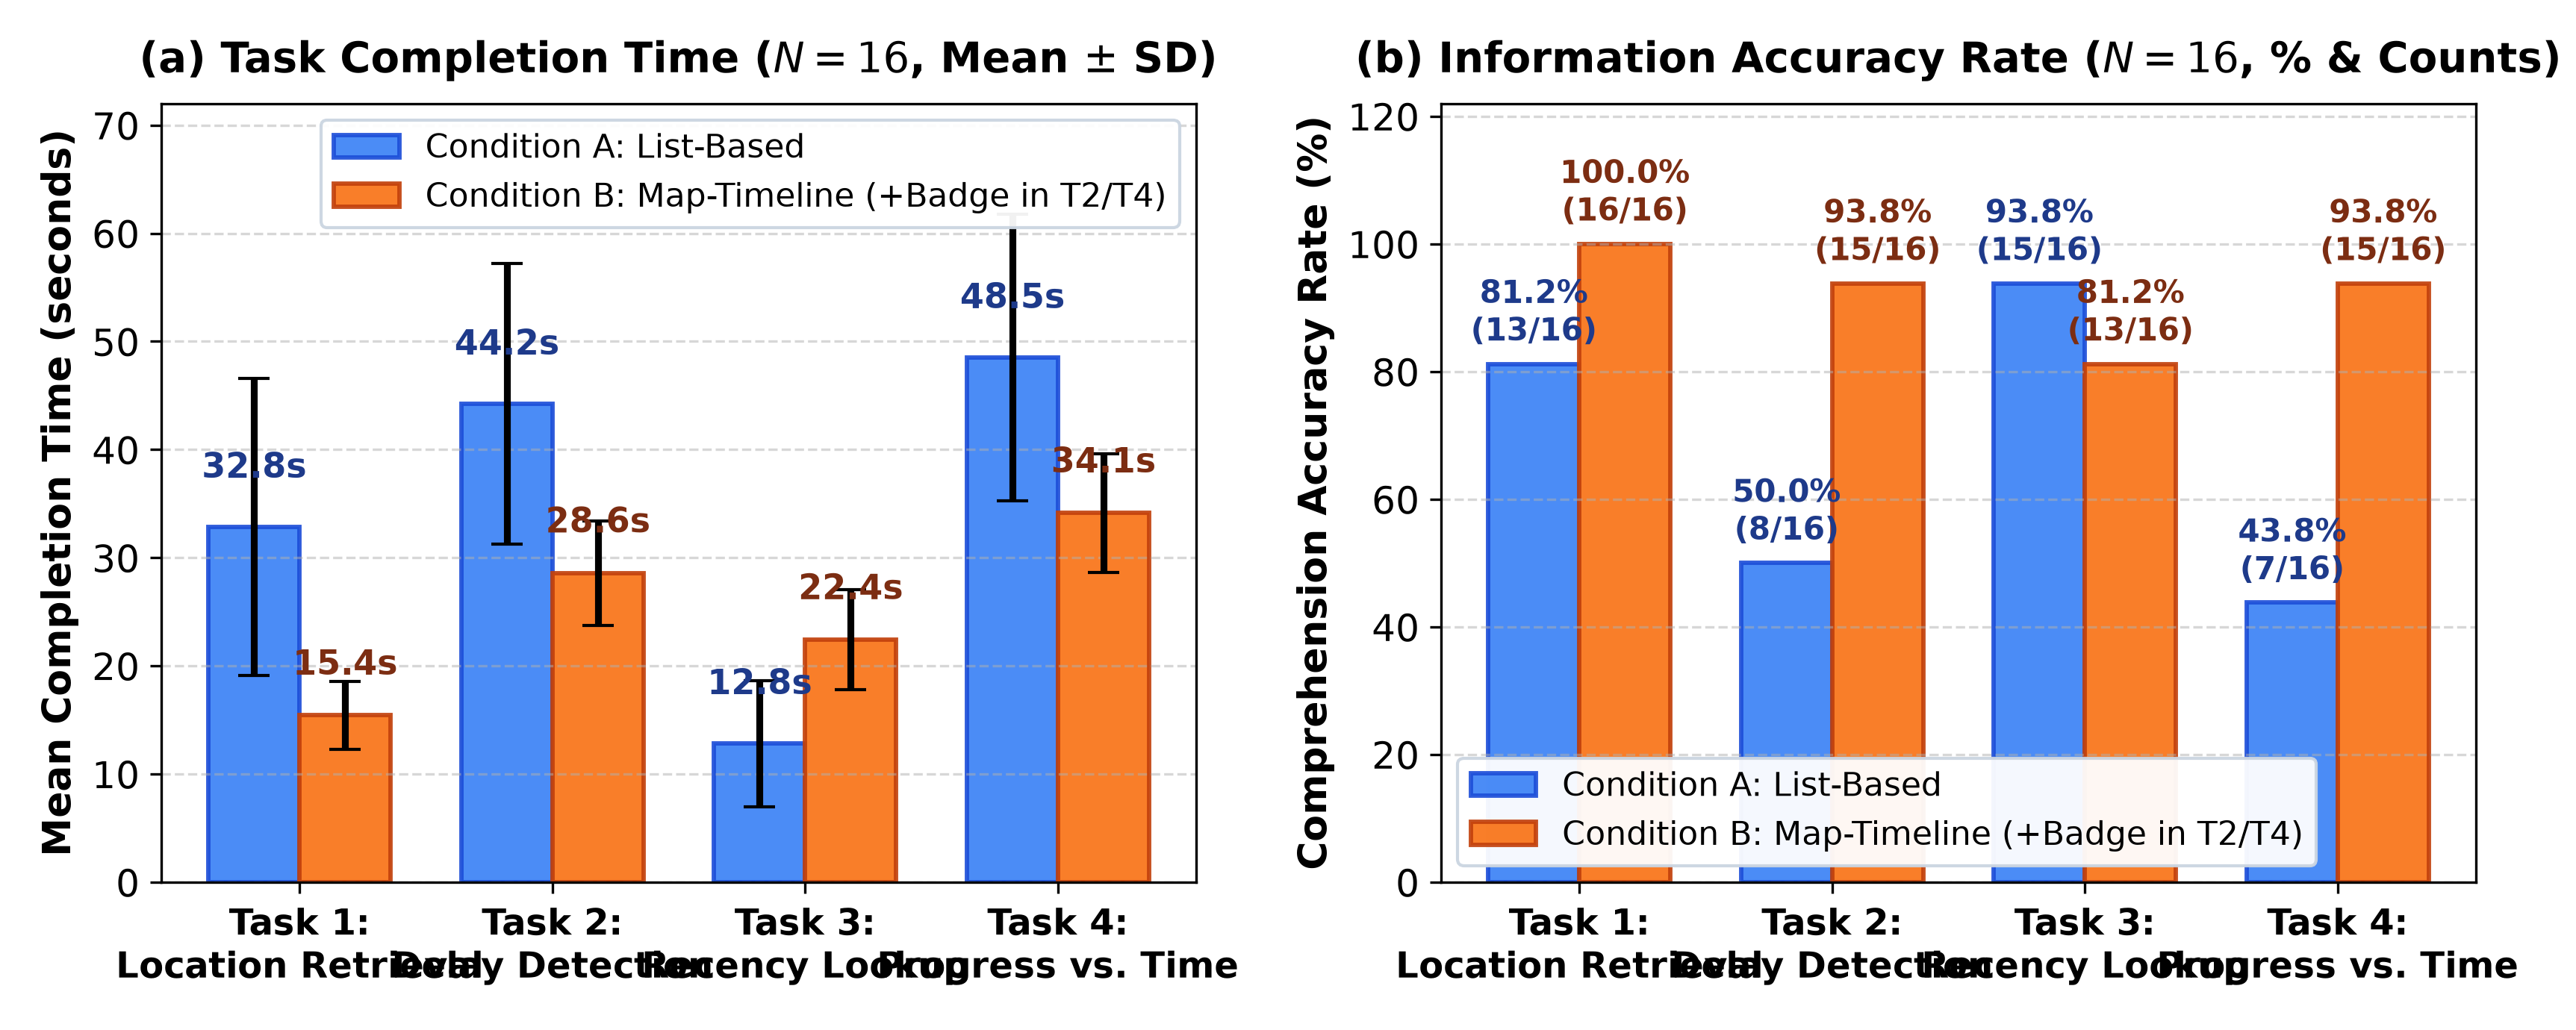
\includegraphics[width=0.60\textwidth]{figures/fig1_task_performance.png}
\caption{Task completion time (seconds) and comprehension accuracy rate across Tasks 1--4 between Condition A (List-Based) and Condition B (Map-and-Timeline) ($N = 16$).}
\label{fig:perf}
\end{figure}

\subsubsection{Spatial Processing vs. Tabular Scanning (Task 1):}
Task~1 strongly corroborated hypothesis $H_{1a}$: the interactive map significantly accelerated spatial project retrieval by 57\% (median 14.05\,s vs. 29.75\,s; paired $t(15) = 5.57, p < 0.001$). For retrieval accuracy ($H_{1b}$), Condition~B achieved a descriptive gain from 81.2\% (13/16) to 100.0\% (16/16). Because accuracy represents paired binary data, an exact two-sided McNemar test was evaluated across discordant pairs ($b = 0, c = 3$), yielding $p = 0.250$. While choropleth visual clustering eliminated serial scanning slips, the accuracy increase remains a descriptive improvement and does not reach statistical significance within this pilot cohort ($N = 16$).

\subsubsection{Mitigation of Schedule Delay Heuristics (Tasks 2 and 4):}
Tasks~2 and 4 supported hypotheses $H_{2a}$ and $H_{2b}$, showing statistically verified gains in both completion time and comprehension accuracy. For task efficiency ($H_{2a}$), the dual-bar timeline significantly cut completion duration by 14--16\,s (Task 2: paired $t(15) = 5.72, p < 0.001$; Task 4: paired $t(15) = 5.33, p < 0.001$). Crucially, the paired binary accuracy gains were statistically confirmed via exact McNemar tests ($H_{2b}$): delay detection accuracy rose significantly from 50.0\% (8/16) to 93.8\% (15/16) in Task 2 ($p = 0.016$; discordant pairs $b = 0, c = 7$), and from 43.8\% (7/16) to 93.8\% (15/16) in Task 4 ($p = 0.008$; discordant pairs $b = 0, c = 8$). In the list condition, participants repeatedly fell victim to the \emph{duration-work equivalence heuristic}, misinterpreting high elapsed time as satisfactory execution. The dual timeline representation coupled with visual variance cues mitigated this bias. \hl{It should be noted that Condition B's explicit ``Terlambat'' delay badge---absent in Condition A by design (Section 3.3)---and its status-coded map pins may themselves contribute to observed accuracy gains in Tasks 2 and 4, independent of the timeline's dual-bar structure. This study cannot fully isolate chronological timeline representation from explicit delay flagging; future work should employ a factorial design varying these two features independently.}

\subsubsection{Interface Complexity Overhead in Elementary Lookups (Task 3):}
Importantly, Task~3 corroborated $H_{3a}$, exposing the operational tax of spatial visual interfaces. When locating a single alphanumeric attribute---the latest field inspection update date---the tabular list was \textbf{significantly faster} (median 12.35\,s vs. 23.85\,s; paired $t(15) = -5.05, p < 0.001$). For accuracy, the tabular list yielded a higher descriptive score (93.8\% [15/16] vs. 81.2\% [13/16]), with an exact McNemar test yielding $p = 0.625$ (discordant pairs: $b = 3, c = 1$). While the accuracy difference was not statistically significant at $N = 16$, the list format imposed lower interaction friction. In the map-and-timeline condition, participants clicked markers, parsed dialogs, and navigated multiple visual panes, with two participants confusing the contract completion deadline with the latest inspection date. This finding is consistent with established GIS-versus-table trade-offs and Cognitive Fit principles~\cite{duncan2021task,bina2023incorporating}.


\subsection{Qualitative Analysis and Cognitive Failure Modes}
Video recordings and think-aloud transcripts were independently coded by two researchers using structured thematic analysis (inter-rater agreement: Cohen's $\kappa = 0.88$). Observed failure modes and anonymized participant statements are categorized in Table~\ref{tab:errors}.

\begin{table}[!htbp]
\centering
\vspace{-3pt}
\caption{Qualitative Failure Modes, Cognitive Mechanisms, and UI Remediation Strategies.}
\label{tab:errors}
\resizebox{\textwidth}{!}{%
\fontsize{7.5pt}{8.6pt}\selectfont
\begin{tabular}{lp{4.2cm}cp{5.2cm}}
\toprule
\textbf{Task Context} & \textbf{Observed Failure Mode} & \textbf{Count ($N=16$)} & \textbf{Participant Statement \& Mechanism} \\
\midrule
\textbf{Task 1}: Spatial Retrieval & Overlooked projects located in target subdistrict on first pass. & 3 / 16 (18.8\%) & \emph{``I missed the Sukodadi row because the text lines blurred together.''} (P06) --- Tabular serial scanning fatigue. \\

\textbf{Task 2}: Delay Detection & Relied on ``In-Progress'' text pill, ignoring negative 19.1\% variance. & 8 / 16 (50.0\%) & \emph{``The badge says In-Progress, so I thought it was progressing fine.''} (P04) --- Semantic priming and duration heuristic. \\

\textbf{Task 3}: Recency Lookup & Reported contract deadline date instead of inspection timestamp. & 3 / 16 (18.8\%) & \emph{``I saw a date at the bottom of the card and thought that was the update.''} (P09) --- Modal visual competition. \\

\textbf{Task 4}: Progress vs. Time & Stated ``elapsed time is 84\%, so project is almost completed.'' & 9 / 16 (56.3\%) & \emph{``84\% means it's almost done, right? Oh, the actual progress is only 67\%.''} (P11) --- Cognitive substitution. \\

\textbf{Study 3}: Missing Data & Inferred null progress indicated project was canceled or 0\%. & 5 / 16 (31.2\%) & \emph{``The cell was empty, so I assumed the government canceled it.''} (P01) --- Negative default inference. \\
\bottomrule
\end{tabular}%
}
\end{table}

\subsection{Evaluation of Missing and Stale Data Perception (Study 3)}
Figure~\ref{fig:study3} summarizes participant cognitive interpretations across the three anomaly scenarios. In Case~1 (\texttt{KTG-PCN-001}, missing progress, update $>150$\,d), 68.8\% (11/16) correctly recognized the data deficiency, while 31.2\% (5/16) misattributed the null field to project cancellation. In Case~2 (\texttt{LMG-SKR-001}, 68\% progress, 117\,d lag), 62.5\% (10/16) recognized that the June report left current status unverified, whereas 37.5\% (6/16) uncritically accepted 4-month-old figures as current reality. In Case~3 (\texttt{KGN-KRN-001}, 55\% progress, 122\,d lag), 75.0\% (12/16) correctly noted unverified status, while 18.8\% overlooked timestamps and 6.2\% assumed work stoppage.

\begin{figure}[!htbp]
\centering
\vspace{-2pt}
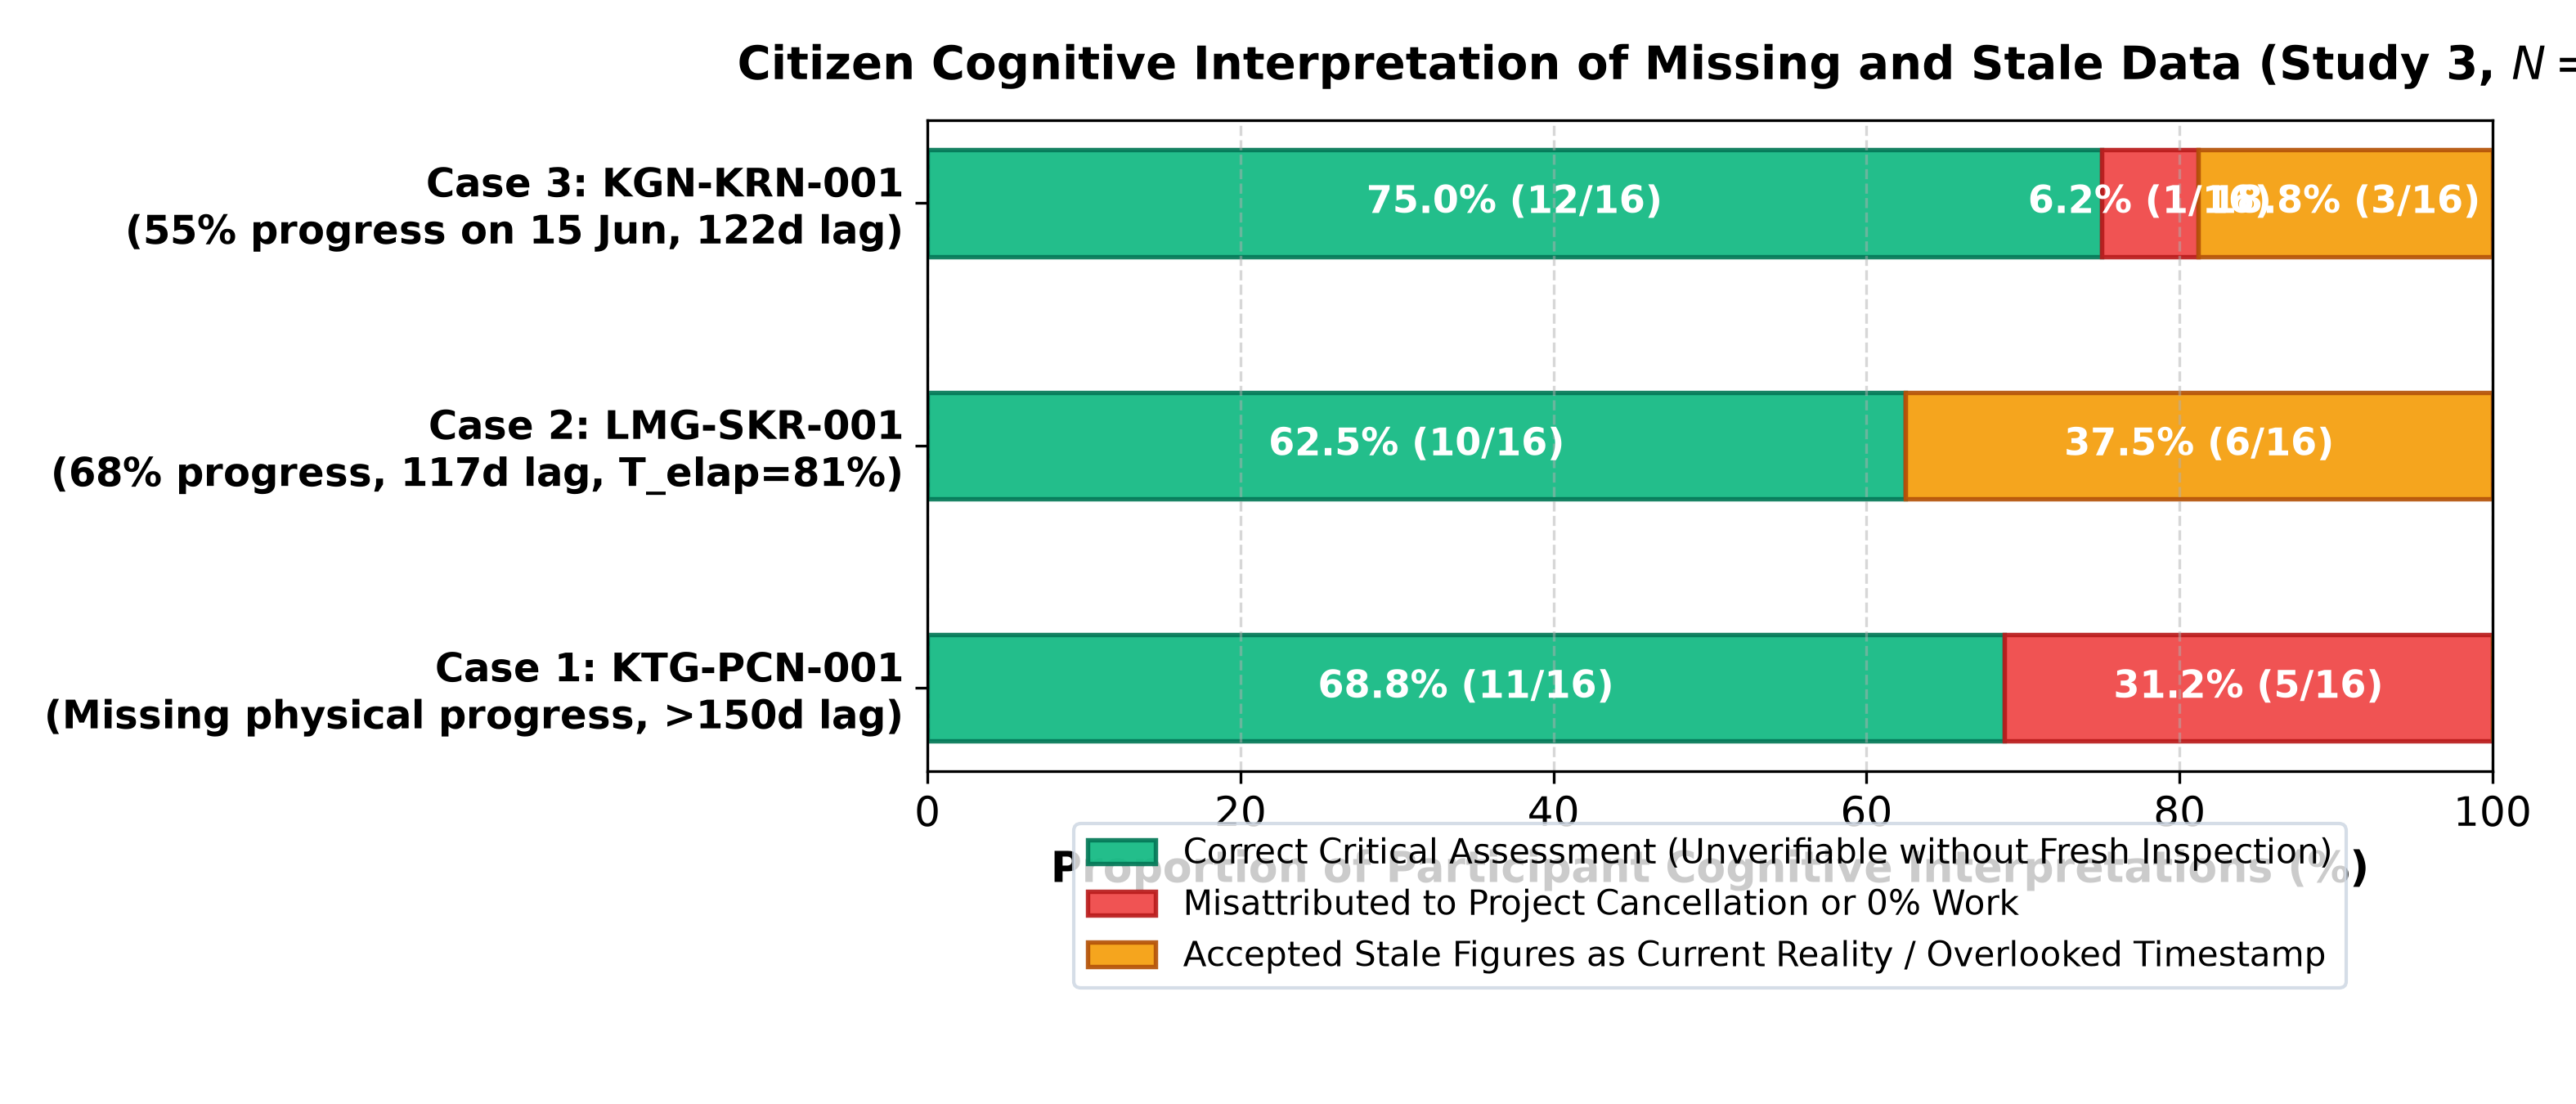
\includegraphics[width=0.46\textwidth]{figures/fig2_missing_stale_perception.png}
\vspace{-3pt}
\caption{Distribution of participant cognitive interpretations under missing and stale reporting conditions (Study 3, $N = 16$).}
\label{fig:study3}
\vspace{-2pt}
\end{figure}

The outcomes of Study~3 demonstrate that \emph{ambiguity breeds false certainty}: 31.2\% (5/16) of participants inferred project cancellation from blank cells, while 37.5\% (6/16) uncritically accepted 4-month-old data as current reality. Civic platforms must implement active freshness badges (e.g., amber warning when updates exceed 60 days) to prevent public misinformation~\cite{ambituuni2025infrastructure,fernstad2022explore}.



\subsection{System Usability Scale (SUS) and Software Quality (ISO/IEC 25010)}
Usability of the CivicTrack integrated platform (\hl{Condition~B; the SUS was not used to compare conditions}) was evaluated using the 10-item System Usability Scale (SUS)~\cite{lewis2021usability}, scored standardly as $\text{SUS} = 2.5 \times [ \sum_{i \in \text{odd}} (S_i - 1) + \sum_{j \in \text{even}} (5 - S_j) ]$ where $S_k \in \{1, \dots, 5\}$ denotes the Likert response for question $k$.

\begin{figure}[!htbp]
\centering
\vspace{-2pt}
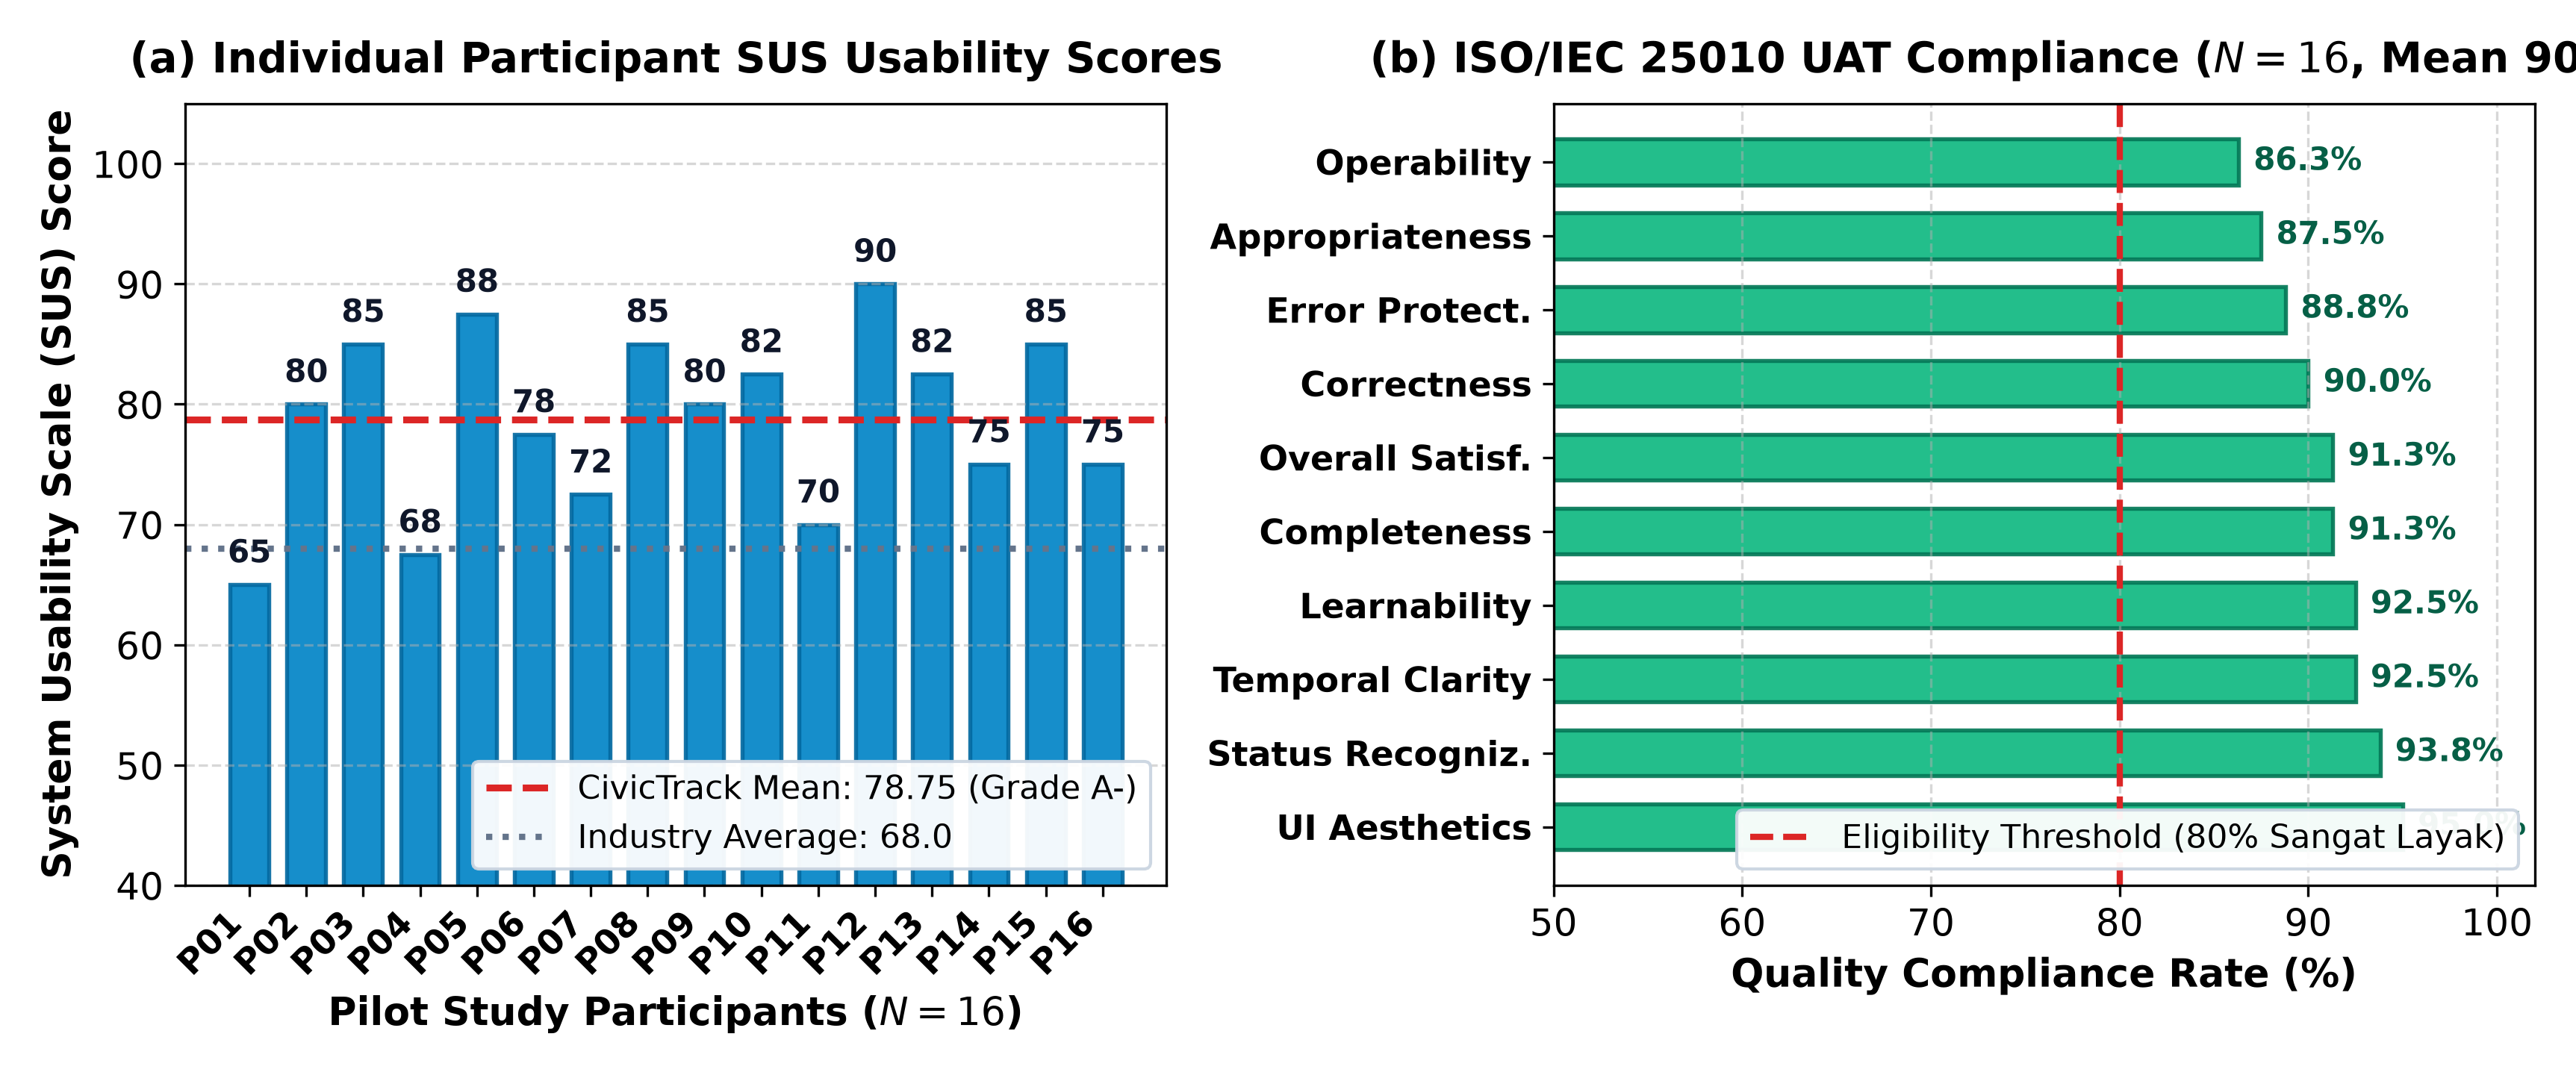
\includegraphics[width=0.46\textwidth]{figures/fig4_combined_usability_quality.png}
\vspace{-3pt}
\caption{System Usability Scale (SUS) individual score distribution and item ratings alongside ISO/IEC 25010 User Acceptance Testing (UAT) quality profile ($N = 16$).}
\label{fig:usability}
\vspace{-2pt}
\end{figure}

As shown in Fig.~\ref{fig:usability}, CivicTrack achieved an overall mean SUS score of \textbf{82.50} ($SD = 4.56$, median 82.50, range 75.0--90.0). This corresponds to \textbf{Grade~A}, ranks at the \textbf{92.5th percentile} of evaluated software systems under empirical benchmark curves~\cite{lewis2021usability,hyzy2022system}, and garners an adjective rating of \textbf{``Excellent''}. Ratings were exceptionally high for ease of navigation ($Q_3$ mean: 4.69/5.00) and learnability ($Q_7$ mean: 4.56/5.00), while operational complexity was minimal ($Q_2$ mean: 1.63/5.00).

In the concurrent ISO/IEC 25010 UAT audit, CivicTrack attained an overall quality rating of \textbf{90.88\%} (727/800 points, \emph{Sangat Layak}). Dimension satisfaction reached 95.00\% for UI Aesthetics, 93.75\% for Appropriateness Recognizability, 92.50\% for Temporal Clarity, and 91.25\% for Functional Completeness. All 95 executed automated test cases (38 Pytest backend and 57 Vitest frontend) passed successfully.


\section{Conclusion}
This pilot study established an empirical evaluation comparing a conventional list-based tabular portal against an integrated map-and-timeline interface. Using a 20-project benchmark modeled on Lamongan Regency, our findings demonstrate clear task-dependent trade-offs:
\begin{enumerate}\setlength{\itemsep}{-1pt}\setlength{\parskip}{0pt}
    \item \textbf{Spatial Scoping:} Geospatial choropleth maps significantly accelerate geographic retrieval by 57\% ($p < 0.001$), accompanied by a descriptive accuracy gain from 81.2\% to 100.0\% ($p = 0.250$).
    \item \textbf{Schedule Comprehension:} \hl{A bundled timeline condition with explicit variance cues significantly reduced completion time ($p < 0.001$) and increased delay detection accuracy from 50.0\% to 93.8\% ($p = 0.016$); because explicit delay badges were absent in Condition A, these gains cannot be attributed to the timeline graphic alone.}
    \item \textbf{Complexity Penalty:} For discrete alphanumeric lookups, tabular lists remain significantly faster ($p < 0.001$), with descriptive accuracy favoring the list format (93.8\% vs. 81.2\%, $p = 0.625$).
    \item \textbf{Data Latency Vulnerabilities:} Omitted or stale data leads over 30\% of citizens to erroneous inferences, mandating explicit visual staleness indicators.
\end{enumerate}

\noindent\textbf{Boundaries of Claims and Limitations:} This study evaluated a pilot cohort of $N = 16$ participants across 128 trials; while statistically robust for cognitive processing metrics, it represents preliminary behavioral evidence. \hl{Furthermore, because Condition B paired graphical timelines with explicit delay badges (``Terlambat'') and status-coded pins while Condition A used uniform ``In-Progress'' labels, observed gains reflect the compound effect of visual timeline structures and explicit semantic flagging rather than timelines in isolation.} Crucially, \textbf{information comprehension is an interface usability metric, not causal proof of corruption reduction or institutional accountability}~\cite{ambituuni2025infrastructure,saelawong2024transparency}. Civic maps and timelines facilitate cognitive access; converting this access into systemic accountability depends on administrative responsiveness, legal whistleblower protections, and civic empowerment. \hl{Future work will extend testing longitudinally across East Java and deploy factorial designs isolating timeline graphics from semantic alert badges.}



%
% ---- Bibliography ----
%
\renewcommand{\doi}[1]{\href{https://doi.org/#1}{\nolinkurl{doi:#1}}}

\bibliographystyle{splncs04}
\bibliography{references}

\end{document}
